\chapter{System Application - Droplet Microluidics}
\section{Aims}
The application of the PDFC to droplet microfluidics serves two purposes. First, it verifies that the system is functioning as intended for use as a research tool. Second, it allows the characterization of droplet formation by a pressure driven flow in conjunction with X and T-junction geometry, an area currently underdeveloped \cite{Christopher2008}. These aims can be fulfilled by the following two objectives:

\begin{enumerate}
\item Determine how applied pressure determine droplet formation regime
\item Relate applied pressure to droplet scaling law \cite{Zhao2011}
\end{enumerate}
\section{Methods}
\subsection{Device Generation}

The T-junction microfluidic device referenced herein is fabricated using standard soft lithography methods \cite{Stroock2002}. Two part Polydimethylsiloxane (PDMS) was poured onto a SU-8 mold previously developed by Schmid and Franke \cite{Schmid2014c} to form an array of individual T-junction channels. The PDMS was cured at 65dC for 3 hours. After cooling to room temperature, the set PDMS was cut and removed from the mold. Tubing connection holes were punched using a standard $0.5mm$ biopsy punch. Next, both glass slide and the PDMS are oxygen-plasma treated, adhered, and exposed to 100dC for 1hour. Prior to use, devices are treated with the aquapel for 10mins, purged with filtered compressed gas and dried at 65dC for 3 hours. 

\subsection{Experimental Procedure}

Droplet formation was captured on a high speed camera at 2.5k to 20k frames per second. The applied control pressure was held constant for the continuous phase at a nominal value of 40, 60 and 80 mbar while varying the discontinuous phase control pressure. Discontinuous phase control pressure was varied at intervals of $\approx$5mbar until droplet formation ceased due to the onset of backflow or instability, for low or high pressures, respectively. The captured images were then analyzed using a custom imageJ script to determine droplet length, $L$, and position, $X$, along an arbitrarily defined axis parallel to the geometry's outlet channel.
 
\section{Results}

For the T-junction channel geometry described the dimensionless droplet ratio of droplet length, $L$, over channel width, $W$, is plotted as a function of the applied control pressure ratios, $\frac{P_{H_2O}}{P_Oil}$, shown in Figure \vref{fig:lwvpr}. Error bars have been calculated by standard deviation of measured droplet length which results in error equal to or smaller than the symbol size and thus not shown.

\begin{figure}[H]
\centering 
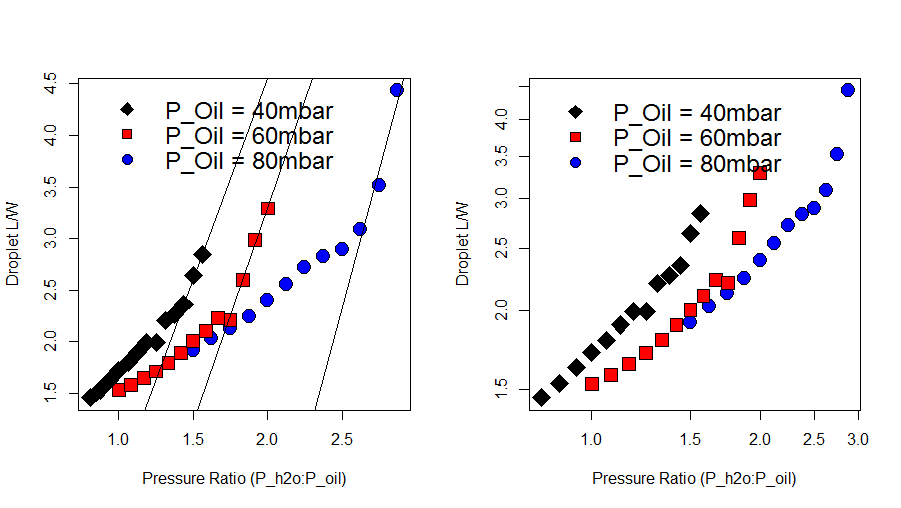
\includegraphics[width=01.0\columnwidth]{lwvpr.PNG} 
\caption[Droplet Length as a Function of Applied Control Pressure Ratio]{Log-log (left) and linear(right) plots of droplet length as a function of the applied control pressure ratio for T-junction geometry.} 
\label{fig:lwvpr} 
\end{figure}

Outer Ca values are calculated given an interfacial tension of $\gamma = 2.87 \times 10^{-3}\frac{N}{m}$, continuous phase viscosity of $\mu = 1.24 \times 10^{-3} Pa \cdot s$\cite{3M2009}, and mean velocity, $u$, as determined by droplet position over consecutive frames as shown in Equation \vref{eq:velocity}.

\begin{equation}
[u] = \Big[\frac{pixels}{frames}\Big] \Big[\frac{frames}{sec}\Big] \Big[\frac{meters}{pixel}\Big] = \Big[\frac{meters}{sec}\Big]
\label{eq:velocity}
\end{equation}

Droplet length is plotted as a function of capillary number as shown in Figure \vref{fig:regimes2} for each of the applied continuous pressures. Images of droplet formation are shown within the squeezing and dripping regimes for each control pressure. The image shown was captured one frame prior to droplet formation. 

\begin{figure}[H]
\centering 
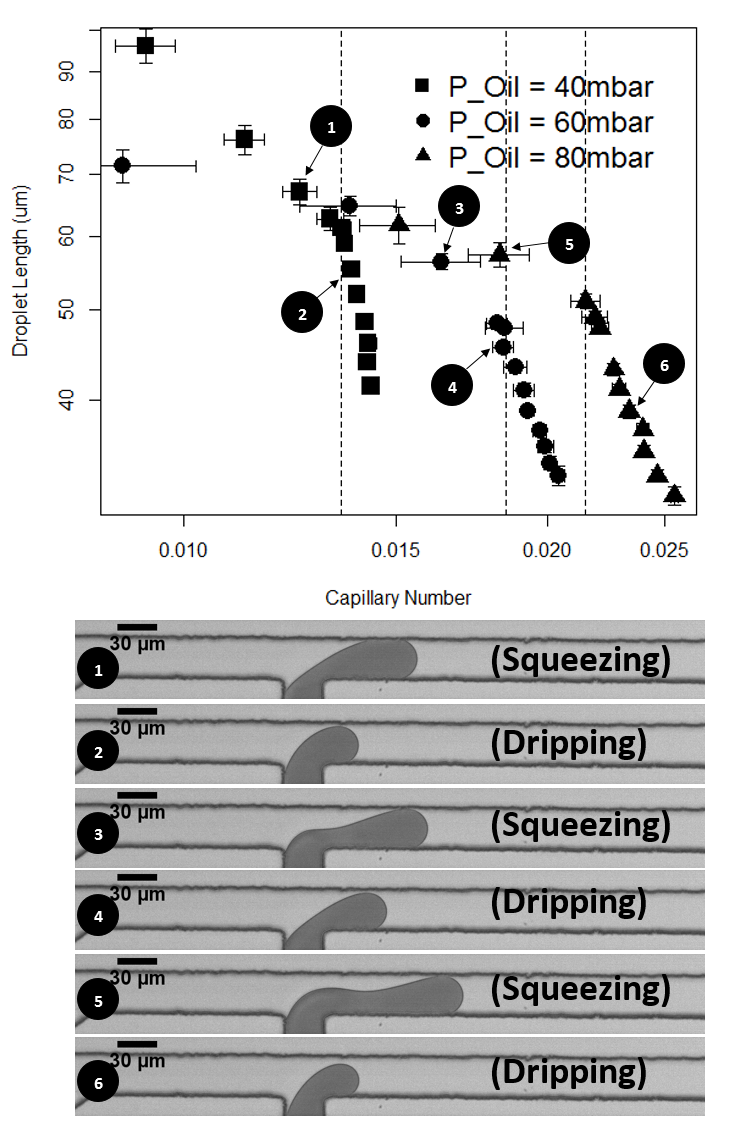
\includegraphics[width=0.75\columnwidth]{regimes2.PNG} 
\caption[Droplet length as a function of Capillary number across squeezing and dripping regimes]{Top: Droplet length as a function of Capillary number across squeezing and dripping regimes, the transition between dripping and squeezing regimes is marked by vertical dashed lines. Bottom: Typical images of droplet elongation just prior to formation.} 
\label{fig:regimes2} 
\end{figure}

Variance in droplet dimensions is analyzed by evaluating the length of droplets formed by constant applied control pressures. Images were acquired at 500 fps for a period of 10 seconds resulting in a sample size of at least 100 droplets with at least three length measurements taken in subsequent frames per unique droplet. A variety
 of investigative plots are shown in Figure \vref{fig:1_poly}, for data acquired at $P_{OIL} = 20mbar,  P_{H_2O} = 80mbar$, resulting in a $Ca$ value of 0.010. The same analysis was conducted at two higher $Ca$ values and is found in Appendix Polydispersity.

\begin{figure}[H]
\centering 
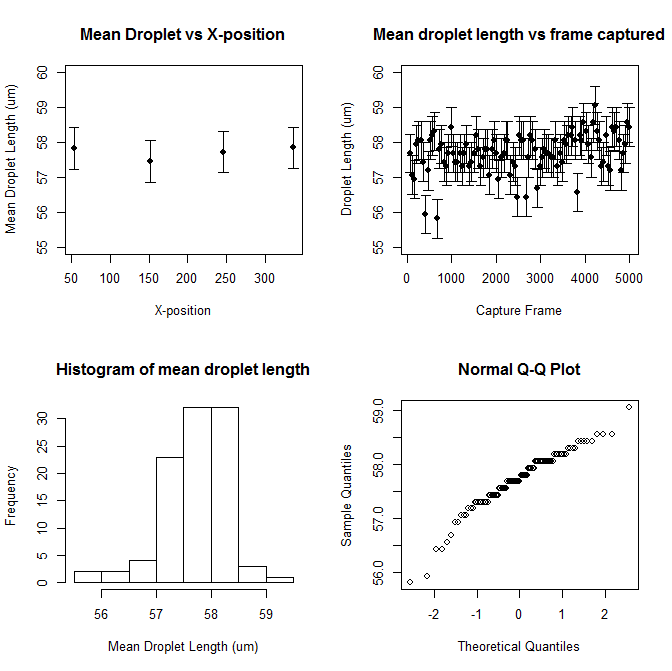
\includegraphics[width=01.0\columnwidth]{1_poly.PNG} 
\caption[Polydispersity]{Distribution of droplet length for P_oil = 0.1bar} 
\label{fig:1_poly} 
\end{figure}


\clearpage

From the analyzed data sets droplet veloctiy, capillary number, mean length, length standard deviation and percent variation ($length stdev / mean length$) are extracted. A summary of the resulting dimensional statistics is shown in Table \vref{tab:poly}.

\qquad

\begin{tabular}{l*{6}{c}r}
P_{Ratio} & Vel (m/s) & Ca & Mean Length(um) & StdDev(um) & Percent Var \\
\hline
4 & 0.023 & 0.010 & 57.71 & 0.55 & 0.95 \\
2.25 & 0.033 & 0.014 & 54.53 & 0.35 &  0.64 \\
1.66 & 0.043 & 0.018 & 48.14 & 0.21 &  0.43 \\
\caption[Droplet Polydispersity]{Dimensional analysis of droplets}
\label{tab:poly} 
\end{tabular}


\clearpage


\section{Discussion}

Previous work has been done to establish specific flow regimes in which droplets are formed in T-junction geometry by both numeric modeling and experimental investigations \cite{Abate2012a},\cite{DeMenech2008},\cite{Garstecki2006}. \emph{However, to the best of the author's knowledge there has been no record of experimental observations demonstrating the regime transition from squeezing to dripping in a pressure-driven flow system.} This, despite the fact that there have been documented dissimilarities in volumetric versus pressure-driven flow in droplet formation\cite{Ward2005}, and that there may be advantages in droplet monodispersity in pressure-driven systems \cite{Christopher2008}\cite{Li2014a}. 

Previous findings suggest that two stable droplet formation regimes exist in T-junction droplet formation, \emph{dripping} and \emph{squeezing}. In a highly cited paper, De Menech et al showed by numerical modeling that the transition between the two distinct droplet regimes may be defined by a Critical Capillary Number, $Ca_{cr}$, and that this transition is independent of viscosity ratio and flowrates, shown in Figure \vref{fig:menechtransition} \cite{DeMenech2008}. This transition has been previously determined both experimentally and in numerical simulations to be $Ca_{cr}\approx 10^{-2}$.

\begin{figure}[H]
\centering 
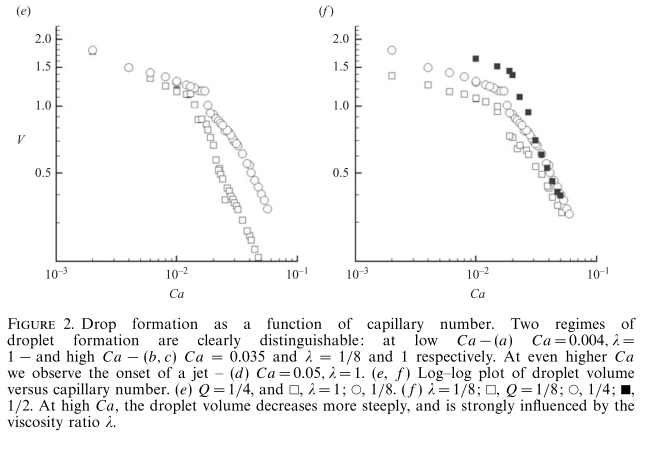
\includegraphics[width=0.75\columnwidth]{menechtransition.PNG} 
\caption[Menech Regime Transition]{Used directly, without permision} 
\label{fig:menechtransition} 
\end{figure}

The data presented here shows a distinct transition between dripping and squeezing regimes, however, the $Ca_{cr}$ value at which the transition occurs is not universal between the different continuous phase pressures. The transitional capillary number can be plotted as a function of the continuous phase pressure as shown in Figure \vref{fig:CrCaABline}.

\begin{figure}[H]
\centering 
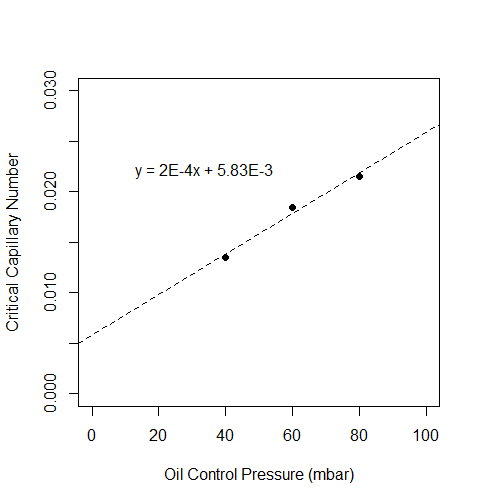
\includegraphics[width=0.75\columnwidth]{CrCaABline.PNG} 
\caption[Critical capillary number as a function of continuous phase applied pressure]{Critical capillary number as a function of continuous phase applied pressure} 
\label{fig:CrCaABline} 
\end{figure}

In these experiments the same bulk reagents are used and therefore both interfacial tension and viscosities should remain constant across multiple trials. Here, the only variable affecting variability in the \emph{Ca} value is the mean velocity of the continuous phase, which in this case is approximated by direct measurement of the droplet velocity. It is expected that there is some numerical difference between the velocity of the droplets and the mean velocity of the continuous phase \cite{Ward2005}, which may account for the variability in critical capillary number.

Unfortunately due to the complex nature of multiphase flow during droplet formation it may be difficult to further investigate the true mean velocity of the continuous phase. However, there is one simplified case that allows for continuous phase flowrate and
\begin{center}

\end{center}
 therefore velocity approximation. That is the case at which no-flow occurs, immediately prior to initial droplet formation within the dripping regime. In this case force balance occurs such that the local continuous phase pressure is equal to the sum of the Laplace pressure and the local discontinuous phase pressure, shown in equation...XX.

\begin{figure}[H]
\centering 
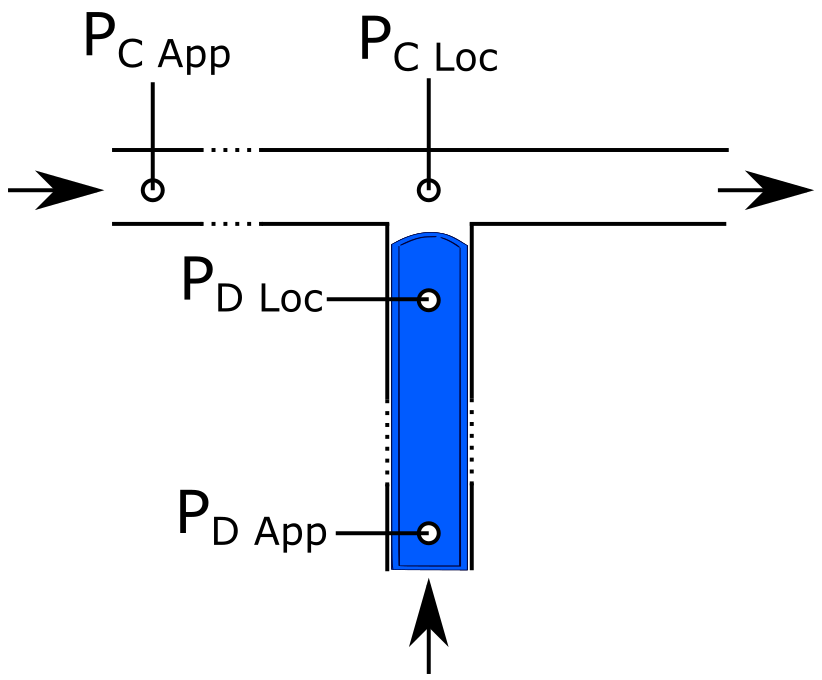
\includegraphics[width=0.75\columnwidth]{pressureBalance.PNG} 
\caption[Pressure Balance at no-flow condition.]{Pressure balance at no-flow condition} 
\label{fig:pressureBalance} 
\end{figure}


A model of Poiseuille flow in a rectangular channel could be used to provide a more accurate determination of the mean continuous phase velocity (as a function of droplet velocity. Alternatively, due to the linear nature of relationship between applied control pressure of the continuous phase and the critical capillary number the velocities could be corrected such that the regime transition is coincident, as shown in Figure \vref{fig:ca_cor}.

\begin{figure}[H]
\centering 
\includegraphics[width=0.75\columnwidth]{Ca_cor.PNG} 
\caption[Corrected capillary number as a function of continuous phase applied pressure]{Corrected capillary number as a function of continuous phase applied pressure} 
\label{fig:ca_cor} 
\end{figure}

In the system developed here, the only inputs used to manipulate flow behavior are the two applied pressures. Therefore, in order to characterize the system's flow regimes it is logical to determine the relationship between applied pressures and the resulting droplet velocity. Here, velocity is plotted as a function of the applied pressure ratio for both T and X-junctions as shown in Figure \vref{fig:vel_pr}.  Ward determined the relationship for their system as shown in Figure \vref{fig:wardVelocity}. (XX we need to do the same)

\begin{figure}[h]
\centering 
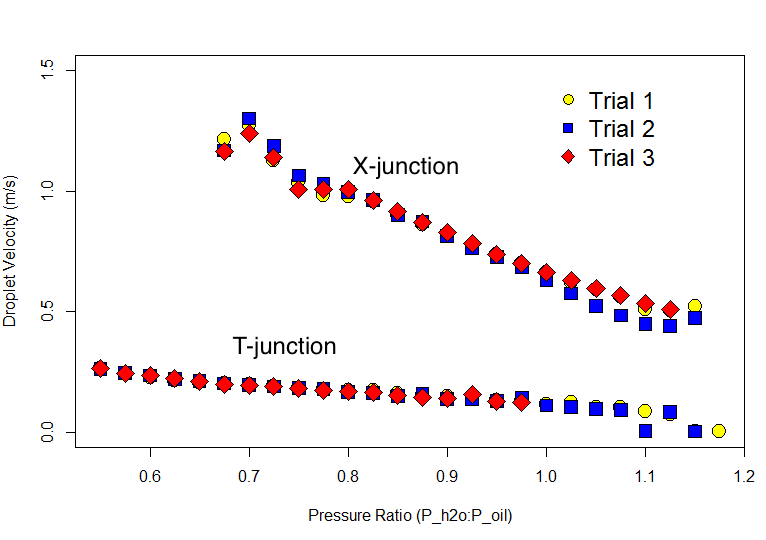
\includegraphics[width=01.0\columnwidth]{vel_pr.PNG} 
\caption[Droplet Velocity as a function of Applied Control Pressure Ratio]{Droplet velocity for both T and X-junctions }
\label{fig:vel_pr} 
\end{figure}


\begin{figure}[h]
\centering 
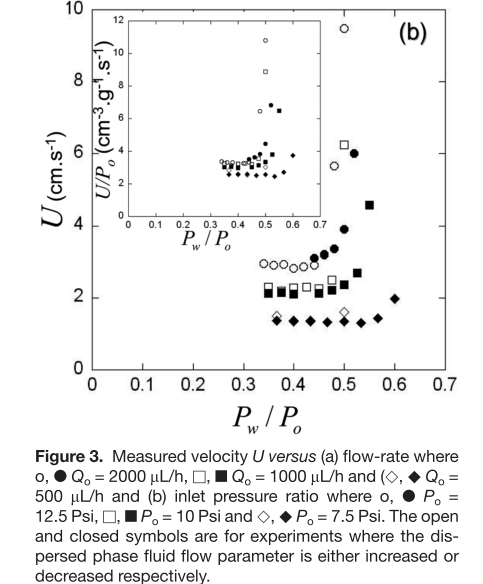
\includegraphics[width=0.75\columnwidth]{wardVelocity.PNG} 
\caption[Velocity, U as a function of applied pressure]{Used without permission, taken directly from \cite{Ward2005} }
\label{fig:wardVelocity} 
\end{figure}



\clearpage

In order to qualitatively characterize the formation of droplets across the entire range of functional pressure ratios, the following section will describe the system behavior at the states of no-flow, dripping, squeezing, and jetting. Due to the strong similarities in droplet-formation behavior between the X-junction and T-junction geometry they will be discussed in general terms with specific metrics given for each case.



\paragraph{No-Flow}
As the system is moved towards the lowest operational pressure ratios, the aqueous phase comes to a a quasi equilibrium no-flow state. As previously reported by Ward et al cite{Ward2005} . If the pressure ratio is decreased any further(either by increasing $P_{Oil}$ or decreasing $P_{H_2O}$) back-flow will occur, in which the continuous phase begins displacing the aqueous phase upstream towards the reservoir. This quasi equilibrium state may be described as a balance of forces between the pressure of the two phases and the Laplace pressure differential across the liquid-liquid interface, described as shown in Equation \vref{eq:noflow}.

\begin{equation}
P_{H_2O*} + P_{Laplace} = P_{Oil*} 
\label{eq:noflow}
\end{equation}

Where Laplace pressure can be roughly approximated given $\gamma$ is the interfacial tension between the two phases, $r$ is the radius of curvature of the interface as:
\begin{equation}
 P_{Laplace} = \frac{2 \gamma}{r}
\label{eq:laplace}
\end{equation}

It should be noted that here $P_{H_2O*}$ and $P_{Oil*}$ represent the pressures of the two phases local to the X or T junction and that there is some unknown pressure drop between the applied control pressures at the inlet reservoirs and these local pressures. This pressure drop is dependent on device geometry as well as solution viscosity and can be determined by Hagan-Poiseuille approximations (XX - needs to be done). 
 
\paragraph{Dripping}

As the control pressure applied to the discontinuous phase is increased beyond the \emph{no-flow} state the immiscible thread begins to extend into the device's channel junction. 


\paragraph{Squeezing}

The pinch point moving further downstream is a manifestation of the increases in tangental viscous forces relative to inertial forces (Ca). The Ca value increases due to the increase in velocity as the interfacial tension and viscosity are both constant. The viscous forces acting tangentially to the discontinuous phase boundary elongates the immiscible thread before the combined effect of increased plugging pressure and inertial forces finally dominate leading to droplet formation.


\begin{comment}
a note on the difference of capillary numbers:
"In microfluidic droplet formation, capillary numbers typically
range from Ca ~ $10^{-3}$ to $10^1$ for flow rates accessible using syringe pumps."\cite{Christopher2007}
\end{comment}



\begin{figure}[h]
\centering 
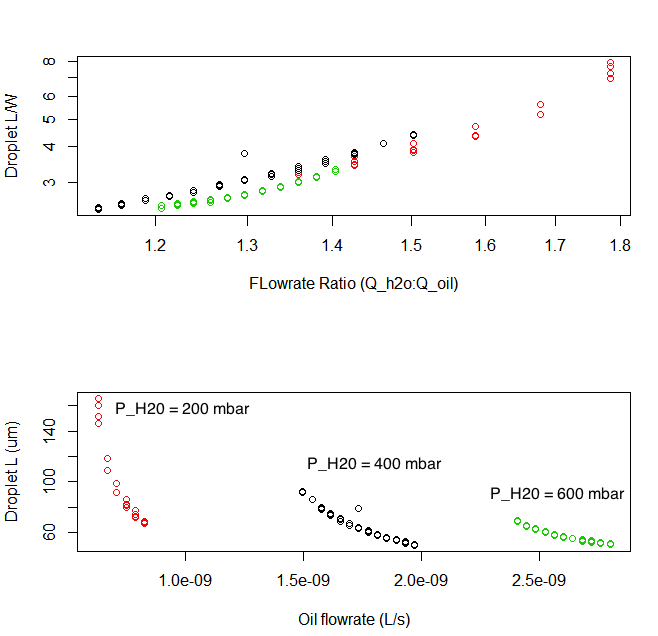
\includegraphics[width=0.750\columnwidth]{constP.PNG} 
\caption[Regime Change at varying flows]{Droplet length at varying flowrates} 
\label{fig:constP} 
\end{figure}


\begin{comment}

Outer Ca values are calculated at the transition between flow regimes given an interfacial tension of $\gamma = 2.87 \times 10^{-3}\frac{N}{m}$, continuous phase viscosity of $\mu = 1.24 \times 10^{-3} Pa \cdot s$, and mean velocities, $u$, as determined by droplet x-position.

\begin{figure}
\centering 
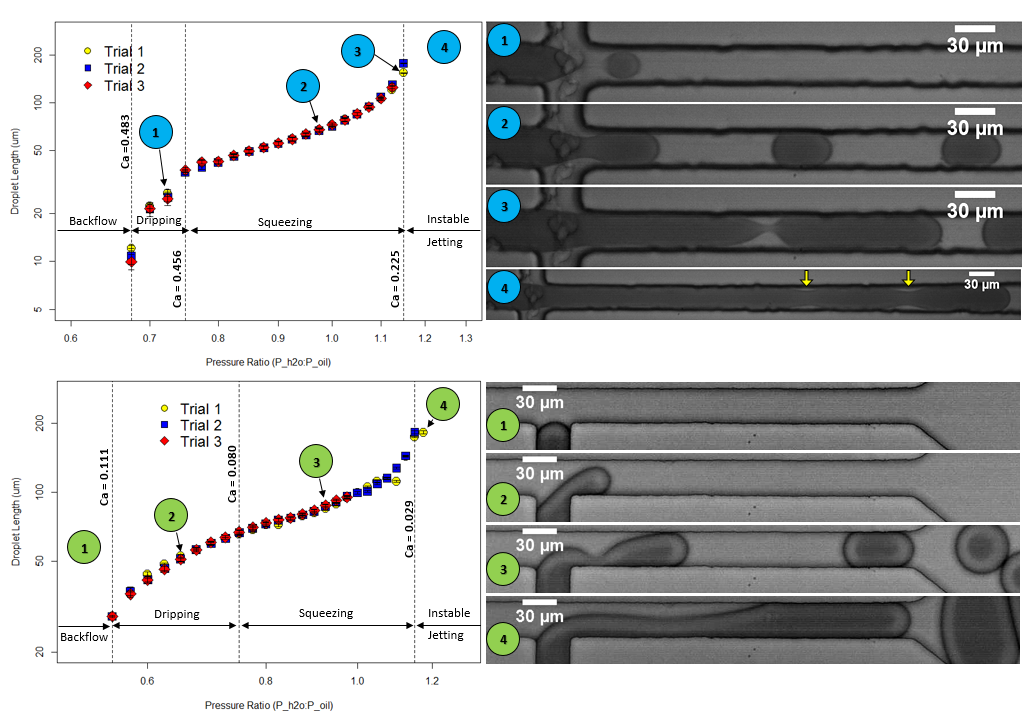
\includegraphics[width=01.0\columnwidth]{regimes.PNG} 
\caption[Droplet Length as a Function of Applied Control Pressure Ratio]{Log-Log plots of droplet length as a function of the applied control pressure ratio for X-junction(top) and T-junction(bottom) geometry. Select images are shown for each geometry showing the case of quasi-equilibrium (bottom-1), droplet formation within the dripping regime (top-1, bottom-2), droplet formation within the squeezing regime (top-2, bottom-3), migration of the 'pinch-point' along the longitudinal axis (top-3, bottom-4), and onset of jetting (top-4).} 
\label{fig:regimes} 
\end{figure}


\end{comment}

